\documentclass[ a4paper, twocolumn]{article}

\usepackage[utf8]{inputenc}
\usepackage{mathtools}
\usepackage{amsmath}
\usepackage{amsthm}
\usepackage{color}
\usepackage{a4wide}
\usepackage{float}
\usepackage{graphicx}
\usepackage{indentfirst}
\usepackage{enumerate}
\usepackage{url}
\usepackage{listings}
\usepackage{caption}

\lstset{
language=Python,
basicstyle=\small\sffamily,
numbers=left,
numberstyle=\tiny,
xleftmargin = 3em,
frame=tb,
columns=fullflexible,
showstringspaces=false,
}

\graphicspath{ {images/} }
\theoremstyle{definition}
\newtheorem{definition}{Definition}[section]

\title{Análise de Algoritmos}
\author{Vinicius A. Matias}
\date{\today}
\begin{document}
\maketitle

\section{Introdução}
Muitos problemas reais podem ser aplicados computacionalmente por meio de algoritmos. A área de análise de algoritmos visa estudar e projetar algoritmos com base no tempo e espaço ocupado para uma solução ótima (de menor custo possível). 

As maneiras mais comuns para medir o custo de algoritmos são: medição direta (medir o tempo de processamento com base no tempo real, logo, é influenciado pelo hardware); custo baseado em um computador ideal (valores tabulados  por linguagem de programação para medir o custo de cada operação); e por meio das operações mais significativas (mais utilizada, focando em identificar as operações que aumentam o custo do algoritmo).

\section{Função de complexidade}

Para a análise de complexidade seguindo a operação de maior custo, podemos definir uma função de complexidade $f(n)$, onde n é o tamanho da entrada e $f(n)$ é o número de comparações necessárias para resolver um problema. Vamos exemplificar o problema utilziando o trecho de código em Python na Listing 1. Este código recebe um vetor ou lista A, que tem tamanho n (determinado por pelo comando \textit{len()}.

\begin{lstlisting}[label=max_array,caption= Maior valor de um arranjo]
def max_array(A):
    max = A[0]
    i = 1
    
    while i < len(A):
        if A[i] > max:
            max = A[i]  
        i += 1
    
    return max
\end{lstlisting}

A operação crítica para este algoritmo é determinada pelo \textit{if} da linha 6, cuja troca pode ser feita, no pior caso, n-1 vezes. Note que antes de se iniciar o loop, max é definido como o primeiro valor do arranjo, consequentemente, é desnecessário utilizar este valor no while (logo, o loop começa do segundo valor e vai até o último, com n-1 comparações). Portante, a função de complexidade para este algoritmo é $f(n) = n - 1, \ \forall \ n>0$. Ainda não foram tratadas as técnicas para definir se um algoritmo é ótimo, mas no caso deste algoritmo, já foi provado que o mínimo de operações necessárias é n-1 (para um arranjo desordenado), logo, este é um algoritmo ótimo.

Projetemos agora um novo algoritmo que calcule o máximo e mínimo de um arranjo no mesmo laço (Listing2). Para desenvolvê-lo reaproveitamos o código do máximo valor em um arranjo e adicionamos uma segunda comparação, caso a primeira tenha falhado (isto é, se o valor na posição atual não for o maior, verificamos se é menor). 

\begin{lstlisting}[label=max_min_array,caption= Maior e menor valor de um arranjo]
def max_min_array(A):
    max = min = A[0]
    i = 1
    
    while i < len(A):
        if A[i] > max:
            max = A[i]
        elif A[i] < min:
            min = A[i]
        i += 1

    return [max, min]
\end{lstlisting}

Pela análise do algoritmo, percebe-se que o melhor caso (menor número de comparações) ocorre quando realizamos apenas o primeiro if, isto é, apenas comparamos o valor atual do arranjo com o maior valor registrado até o momento. Este caso ocorre quando o arranjo é passado ordenado, logo, o valor mínimo nunca será alterado e o valor máximo sempre será trocado, resultando em $n-1$ operações. 

O pior caso é quando realizamos a segunda operação em todas as iterações. Para isto acontecer basta que o primeiro valor do arranjo seja o valor máximo, portanto, o primeiro teste sempre irá falhar e o segundo sempre será executado.   Importante notar que o pior caso inclui o arranjo em ordem decrescente, mas não somente. Dado que o laço corre $n-1$ vezes e realizamos duas comparações nele, nosso algoritmo tem $f(n) = 2(n-1)$. Novamente, tanto o melhor caso quanto o pior caso são dados para todo $n>0$.

Tipicamente, estamos interessados em identificar o custo do algoritmo no pior caso, mas técnicas para determinar a complexidade de algoritmos no caso médio, melhor e pior caso serão discutidas nos próximos tópicios.

\subsection{Exercícios}
1. Determine a função de complexidade da busca sequêncial de um vetor A d tamanho n para o melhor caso, pior caso e caso médio.

Resolução: 

\begin{itemize}
\item Pior caso: a busca passará pelos n elementos, logo, $f(n) = n$
\item Melhor caso: o primeiro elemento é o valor buscado, logo, $f(n) =  1$
\item Caso médio: Para este problema, podemos dizer que devemos passar por 50\% dos elementos para encontrar o valor, portanto $f(n) = n/2$
\end{itemize}

\begin{lstlisting}[label=linear_search,caption= Busca sequêncial]
def linear_search(A, target):
    n = len(A)

    for i in range(n):
        if A[i] == target:
            return i
    
    return -1
\end{lstlisting}

\section{Crescimento Assintótico}
Como já deve ter ficado claro, as funções de complexidade dependem de n, o que deve ser o responsável por aumentar o tempo de execução do algoritmo. A tabela 1 mostra o cresimento na quantidade de operações para três n's em três diferentes funções de complexidade. O algoritmo para retornar os valores da tabela foi construído em R.

\begin{table}[H]
\caption{\label{tab:crescimento}Comportamento Assintótico}
\begin{tabular}{l*{6}{c}r}
	 & 100 & 1000 & $10^6$ \\
	\hline
	$\log n$ & 2 & 3 & 6 \\
	$n$ & 100 & 1000 & 1e+06 \\
	$n \log n$ & 200 & 3000 & 6e+06 \\
	$n^2$ & 1e+04 & 1e+06 & 1e+12 \\
	$100n^2$ + 15n & 1e+06 & 1e+08 & 1e+14 \\
	$2^{n}$ & 1.3e+30 & 1e+301 & Inf \\
\end{tabular}
\end{table}

Note que a entrada \textit{n} sempre aumentará a quantidade de operações, mas a função de complexidade interfere muito mais no aumento do custo. Na análise da complexidade dos algoritmos nos interessará encontrar, por exemplo, a partir de qual valor de n uma função se torna maior que outra (ou, em palavras bonitas, quando uma função domina assintóticamente outra função). Veja na figura 1 um exemplo. Caso necessário, dê zoom na imagem, mas o eixo x representa os valores de n(0 à 100) e y a quantidade de operações. A partir de n = 5 a função vermelha passa a crescer mais que a função azul mediante o aumento do n. À título de curiosidade, a função vermelha cresce em $x^3$ e a função azul cresce em $5x$.

\begin{figure}[h]
\begin{center}
	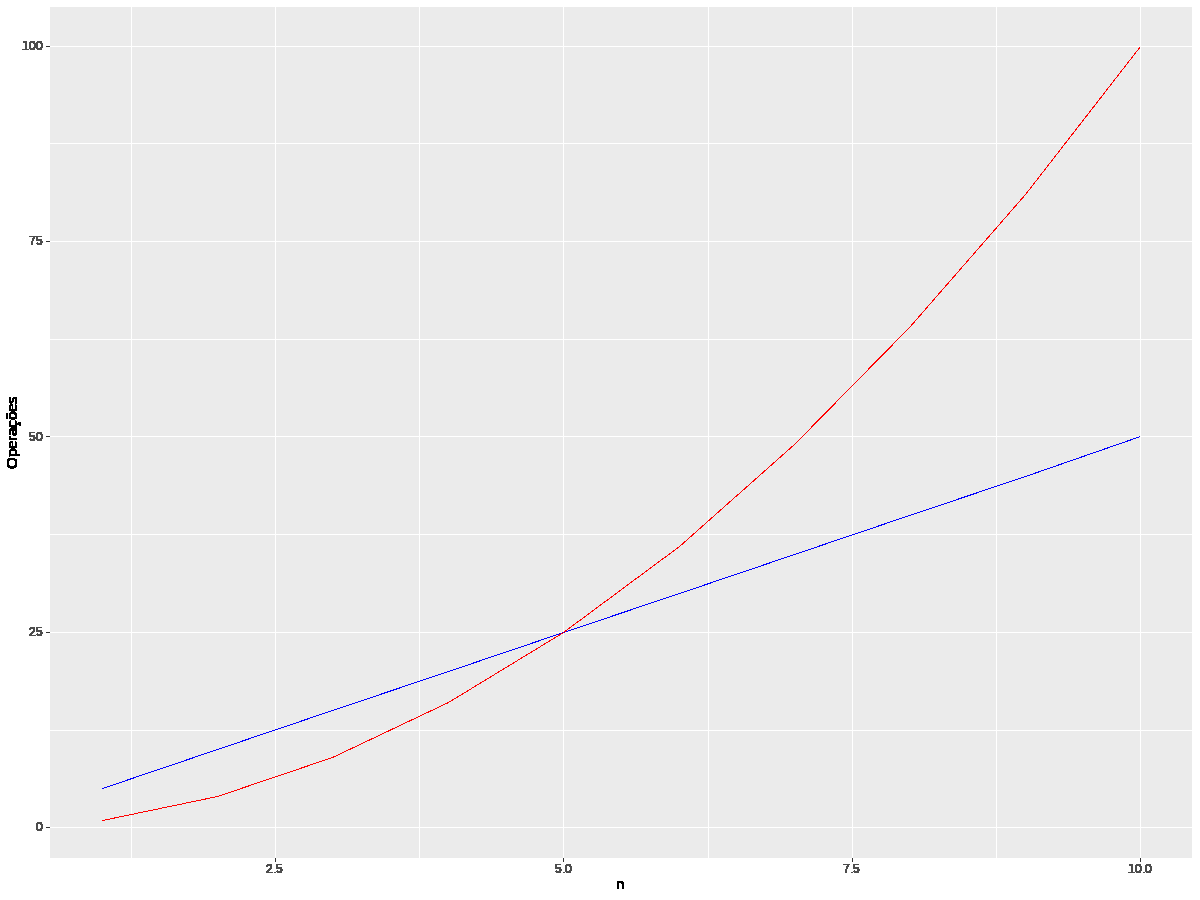
\includegraphics[width=7cm]{grow.png}
	\caption{Crescimento no número de operações para diferentes valores de n em duas funções de complexidade}
\end{center}
\end{figure}


\section{Notação $\mathcal{O}$}
A notação $\mathcal{O}$ (leia-se O grande ou Big-O) diz que $f(n)$ cresce no máximo ou tanto quanto $g(n)$ pela notação $f(n) = \mathcal{O}(g(n))$. 

\begin{definition}
$\mathcal{O}(g(n)) = \{f(n)$: existem constantes positivas $c$ e $n_0$ tais que $0 \leq f(n) \leq cg(n)$, para todo $n \geq n_0$\}
\end{definition}

\subsection{Exemplo}
Demonstrar que $f(n) = \frac{3}{2}n^2 - 2n \in \mathcal{O}(n^2)$. 

Isso é o mesmo que dizer que existem constantes positivas $c$ e $n_0$ onde: 
$0 \leq f(n) \leq cg(n)$

Resolvendo $0 \leq f(n)$:

\begin{enumerate}[Step 1:]
\item $0 \leq \frac{3}{2}n^2 - 2$

\item $0 \leq n(\frac{3}{2}n - 2)$

Como n  $\geq$ 0, a multiplicação $n(\frac{3}{2}n - 2)$ vai ser maior ou igual à zero se $\frac{3}{2}n - 2$ for maior ou igual à zero. Resolvendo essa multiplicação temos: 

\item $0 \leq \frac{3}{2}n - 2n$

\item $2 \leq \frac{3}{2}n$

\item $\frac{2}{3/2} \leq n$

\item $\frac{4}{3} \leq n$

Logo, $n$ deve ser maior ou igual à $4/3$

\end{enumerate}

Resolvendo $\frac{3}{2}n^2 - 2n  \leq cn^2$ (note que $g(n) = n^2$ para $\mathcal{O}(n^2)$:

\begin{enumerate}[Step 1:]
\item $\frac{3}{2}n^2 - 2n \leq cn^2$

\item $n(\frac{3}{2}n - 2) \leq cn^2$

\item $\frac{3}{2}n - 2 \leq cn$

\item $- 2 \leq cn - \frac{3}{2}n$

\item $cn - \frac{3}{2}n \geq -2$

\item $n(c - \frac{3}{2}) \geq -2$

Como n  $\geq$ 0, a multiplicação $n(c - \frac{3}{2})$ é maior ou igual que -2 quando $(c - \frac{3}{2}) \geq 0$

\item $c - \frac{3}{2} \geq 0$

\item $c \geq \frac{3}{2}$

Logo, $c \geq 3/2$ e $n \geq 0$

\end{enumerate}

Como $n \geq 4/3, n \geq 0 e c \geq 3/2$, podemos escolher constantes $n_0$ e $c$ que satisfaçam essas condições. Como exemplo:

$ n_0 = 2, c = 3/2$

\section{Notação $\Omega$}
A notação $\Omega$ (Omega) significa que $f(n)$ cresce mais ou tão rápido quanto $g(n)$, ou que $f(n)$ domina $g(n)$

\begin{definition}
$\Omega (g(n)) = \{f(n)$: existem constantes positivas $c$ e $n_0$ tais que $0 \leq cg(n) \leq f(n)$, para todo $n \geq n_0$\}
\end{definition}


\subsection{Exemplo}
Demonstrar que $f(n) = \frac{3}{2}n^2 - 2n \in \Omega(n^2)$. 

Isso é o mesmo que dizer que existem constantes positivas $c$ e $n_0$ onde: 
$0 \leq cg(n) \leq f(n)$

Resolvendo $0 \leq cg(n)$:


\begin{enumerate}[Step 1:]
	\item $0 \leq cn^2$
	
	Se $n \geq 0$, a condição também é satisfeita para $c \geq 0$
	
\end{enumerate}

Resolvendo $cg(n) \leq f(n)$

\begin{enumerate}[Step 1:]	
	\item $cn^2 \leq \frac{3}{2}n^2 - 2n$
		
	\item $cn^2 \leq n(\frac{3}{2}n - 2)$	
	
	\item $cn \leq \frac{3}{2}n - 2$
	
	\item $2 \leq \frac{3}{2}n - cn$
	
	\item $2 \leq n(\frac{3}{2} - c)$
	
	Como n e c são maiores que 0, a inequação será verdadeira para $(\frac{3}{2} - c) > 0$ e um consequente valor mínimo de n.
	
	\item $(\frac{3}{2} - c) > 0 \rightarrow c < \frac{3}{2}$
	
	Como precisamos de um $c < 3/2$, consideraremos c = 1 aplicado ao passo 5
	
	\item $2 \leq n(\frac{3}{2} - 1)$
	
	\item $2 \leq n(\frac{1}{2})$

	\item $4 \leq n \rightarrow n \geq 4$
	
	Logo, $\frac{3}{2}n^2 - 2n \in \Omega(n^2)$ para $n_0 = 4$ e $c = 1$
		
\end{enumerate}

\section{Notação $\Theta$}
A notação $\Theta$ (Theta) diz que uma função de complexidade $f(n)$ cresce no mínimo tão lentamente quanto $c_1g(n)$ e no máximo tão rapidamente quanto $c_2g(n)$, logo, $f(n)$ deverá crescer junto à $g(n)$, ou seja, tão rapidamente quanto $g(n)$.

\begin{definition}
	$\Theta(g(n)) = \{f(n)$: existem constantes positivas $c_1$, $c_2$ e $n_0$ tais que $0 \leq c_1g(n) \leq f(n) \leq c_2g(n)$, para todo $n \geq n_0$\}
\end{definition}

Note que $0 \leq c_1g(n) \leq f(n)$ é a definição de $\mathcal{O}$ para um $c = c_1$ ($f(n)$ domina $g(n)$), e que $0 \leq f(n) \leq c_2g(n)$ é a definição de $\Omega$ para $c = c_2$ ($g(n)$ domina $f(n)$). A partir disso pode-se concluir duas coisas. 

A primeira conclusão é algo que foi mencionado no parágrafo anterior à definição: $\Theta(g(n))$ significa que uma função cresce tão rapidamente quanto $g(n)$. Se $f(n)$ domina e é dominado por $g(n)$, $f(n)$ deve crescer tão rapidamente quanto $g(n)$.

A segunda conclusão é que para definir as constantes de $\Theta(g(n))$, podemos utilizar as constantes $c$ e $n_0$ encontradas em $\mathcal{O}(g(n))$ e $\Omega(g(n))$, tomando o cuidado de se escolher um $n_0$ que satisfaça as condições de $\mathcal{O}(g(n))$ e $\Omega(g(n))$.

\subsection{Exemplo}
Demonstrar que $f(n) = \frac{3}{2}n^2 - 2n \in \Theta(n^2)$. 

Isso é o mesmo que dizer que existem constantes positivas $c_1$, $c_2$ e $n_0$ onde: 

$0 \leq c_1g(n) \leq f(n) \leq c_2g(n)$

Como $cf(n) \in \mathcal{O}(g(n)) $ para $c = \frac{3}{2}$ e $n_0 = 2$; e

$cf(n) \in \Omega(g(n))$ para $c = 1$ e $n_0 = 4$

Podemos concluir que $f(n) = (3/2)n^2 - 2n \in \Theta(n^2)$ para $c_1 = 1$, $c_2 = 3/2$ e $n_0 = 4$.

\section{Notação o}
A notação $o(g(n))$ ("o" minúsculo ou "o" pequeno)  diz que uma função $f(n)$ cresce mais lentamente que $g(n)$.

\begin{definition}
	$o(g(n)) = \{f(n): \forall c>0, \ \exists \ n_0 > 0 \ | \ 0 \leq f(n) < cg(n), \ \forall n \geq n_0 \}$
\end{definition} 

\subsection{Exemplo}
Demonstrar que $1000n^2 \in o(n^3)$ (uma função quadrática cresce mais lentamente que uma função cúbica)

Demonstrar que $f(n) \in o(g(n)))$ é o mesmo que mostrar que para toda constante positiva c, existe um valor de $n_0 > 0$ que satisfaça a inequação $0 \leq f(n) < cg(n)$

Logo, deve-se encontrar uma função de $n_0$ em relação à $c$ para $0 \leq 1000n^2 < cn^3$

Resolvendo $0 \leq 1000n^2$ identificamos que o resultado é válido para qualquer valor real de $n$.

Resolvendo $1000n^2 < cn^3$:

\begin{enumerate}[Step 1:]
	\item $1000n^2 < cn^3$
	\item $1000 < cn$	
	\item $1000/c < n$
	\item $n > 1000/c$
	
	Dada esta inequação, precisamos formular uma equação para $n_0$ que siga as diretrizes de n estritamente maior que 1000/c. Uma equação possível é $n_0 = \frac{1000}{c} + 1$.
\end{enumerate}
Assim, encontramos uma função de $n_0$ em função de c que satisfaz $0 \leq 1000n^2 < cn^3$, sendo essa a função $n_0 = \frac{1000}{c} + 1$.

\section{Notação $\omega$}
A notação $\omega(g(n))$ (ômega pequeno)  diz que uma função $f(n)$ cresce mais rapidamente que $g(n)$.

\begin{definition}
	$o(g(n)) = \{f(n): \forall c>0, \ \exists \ n_0 > 0 \ | \ 0 \leq cg(n) < f(n), \ \forall n \geq n_0 \}$
\end{definition} 

\subsection{Exemplo}
Demonstrar que $\frac{n^2}{1000} \in \omega(n)$ (uma função quadrática cresce mais rapidamente que uma função linear)

Demonstrar que $f(n) \in \omega(g(n)))$ é o mesmo que mostrar que para toda constante positiva c, existe um valor de $n_0 > 0$ que satisfaça a inequação $0 \leq cg(n) < f(n)$

Logo, deve-se encontrar uma função de $n_0$ em relação à $c$ para $0 \leq cn < \frac{n^2}{1000}$

Resolvendo $0 \leq cn$ identificamos que o resultado é válido para qualquer valor positivo de $n$ e $c$.

Resolvendo $cn < \frac{n^2}{1000}$

\begin{enumerate}[Step 1:]
	\item $cn < \frac{n^2}{1000}$
	\item $c < \frac{n}{1000}$
	\item $1000c < n \rightarrow n > 1000c$
	
	Dada esta inequação, precisamos formular uma equação para $n_0$ que siga as diretrizes de n estritamente maior que 1000c. Uma equação possível é $n_0 = 1000c + 1$.
\end{enumerate}
Assim, encontramos uma função de $n_0$ em função de c que satisfaz  $0 \leq cn < \frac{n^2}{1000}$, sendo essa a função $n_0 = 1000c + 1$.

\end{document}